\documentclass[../main.tex]{subfiles}

\begin{document}
    \subsection{Keyboard and Mouse Models}

    We managed to achieve impressive results with our keyboard and mouse models, considering how unintuitive the connection between
    mouse and keyboard dynamics and user feelings seems. To start, we can look at this table \ref{table:shoham_models}, 
    which compares all the models trained for one of the participants. We can immediately see that most models have similar performance, 
    with logistic regression being the best. This table was an example of just one participant, one duration, and one labeling type. 

    \begin{table}[htp]
        \centering
        \begin{center}
            \begin{tabular}{cccc}
                \toprule
                model &  accuracy & balanced accuracy & \\
                \midrule
                    majority rule           & 0.2220 & 0.1670 & \\
                    AdaBoost                & 0.4220 & 0.3680 & \\
                    bagging                 & 0.4220 & 0.3780 & \\
                    decision\_tree          & 0.3780 & 0.3400 & \\
                    knn                     & 0.3560 & 0.3140 & \\
                    linear\_svm             & 0.4000 & 0.3540 & \\
                    logistic\_regression    & 0.4220 & 0.4130 & \\
                    random\_forest          & 0.3560 & 0.3170 & \\
                    voting ensamble         & 0.3780 & 0.3400 & \\
                \bottomrule
            \end{tabular}
        \end{center}
        \caption{Results of models trained with one participants data, using both mouse and keyboard, duration 10 and categorical labels.}
        \label{table:shoham_models}
    \end{table}


    To ensure that our models can significantly improve upon a baseline model, 
    we have taken the best model trained for each person with a specific labeling type and duration and calculated a confidence interval 
    for the difference between the best metric and the baseline metric. We can see some of the results in the charts here \ref{fig:cat_val_5_10}. 
    More charts can be found in the appendix \ref{appendix:additional_results}.

    \begin{figure}
        \centering
        \begin{subfigure}[b]{0.42\textwidth}
            \centering
            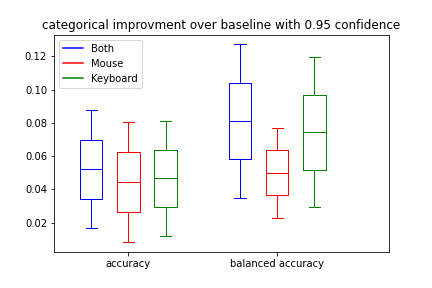
\includegraphics[width=\textwidth]{figures/results/1_categorical_0.95.png}
            \captionsetup{justification=centering}
            \caption{Confidence interval calculated for models using duration of 1 and predicting categorical labels.}
            \label{fig:cat_1}
        \end{subfigure}
        \hfill
        \begin{subfigure}[b]{0.42\textwidth}
            \centering
            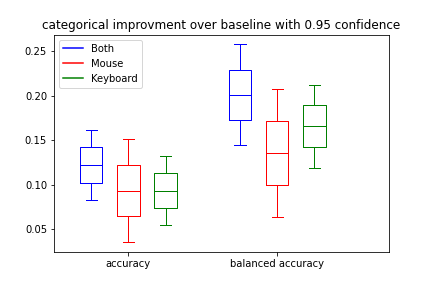
\includegraphics[width=\textwidth]{figures/results/10_categorical_0.95.png}
            \captionsetup{justification=centering}
            \caption{Confidence interval calculated for models using duration of 10 and predicting categorical labels.}
            \label{fig:cat_10}
        \end{subfigure}
        \begin{subfigure}[b]{0.42\textwidth}
            \centering
            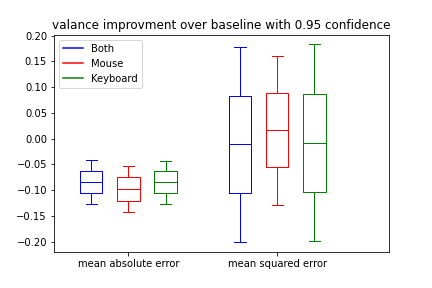
\includegraphics[width=\textwidth]{figures/results/1_valance_0.95.png}
            \captionsetup{justification=centering}
            \caption{Confidence interval calculated for models using duration of 1 and predicting valance labels.}
            \label{fig:val_1}
        \end{subfigure}
        \hfill
        \begin{subfigure}[b]{0.42\textwidth}
            \centering
            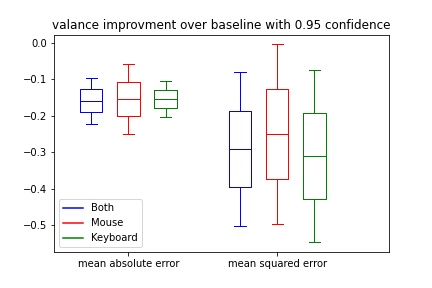
\includegraphics[width=\textwidth]{figures/results/10_valance_0.95.png}
            \captionsetup{justification=centering}
            \caption{Confidence interval calculated for models using duration of 10 and predicting valance labels.}
            \label{fig:val_10}
        \end{subfigure}
        \caption{Confidence interval charts for valance and categorical labels.}
        \label{fig:cat_val_5_10}
    \end{figure}

    Additionally, we can see that the higher duration models improve upon the baseline more consistently, 
    and the improvement seems better when we look at the balanced accuracy, which indicates that the models do indeed learn to predict uncommon labels. 
    We can also notice that the mouse seems a little better than the keyboard usually, and surprisingly models using both are consistently better than either. 

    Finally, we can also say that the models we trained have consistent results across different people, both in the raw accuracy numbers as we see in 
    \ref{appendix:additional_results} and in the confidence intervals, we can notice that the interval is small. For example, when looking at a duration of 10, 
    usually, the interval is smaller than 0.05 for classification models.
    We can see this more clearly for categorical labels here \ref{fig:categorical_kbm}

    \begin{figure}
        \centering
        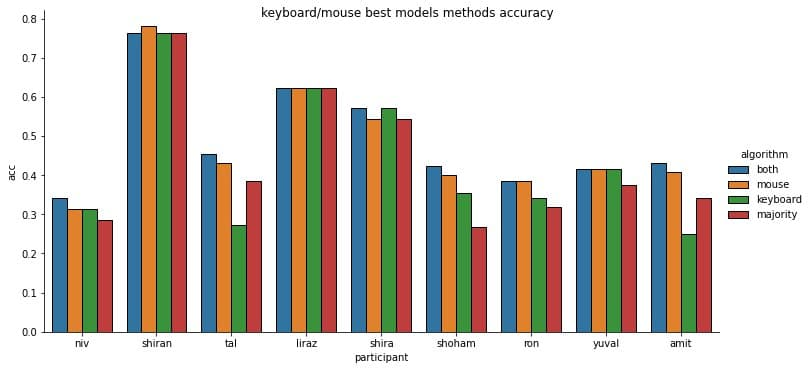
\includegraphics[width=14cm]{figures/results/categorical_kbm}   
        \caption{Here we can see a comparison of the the best models}
        \label{fig:categorical_kbm} 
    \end{figure}

    \begin{figure}
        \centering
        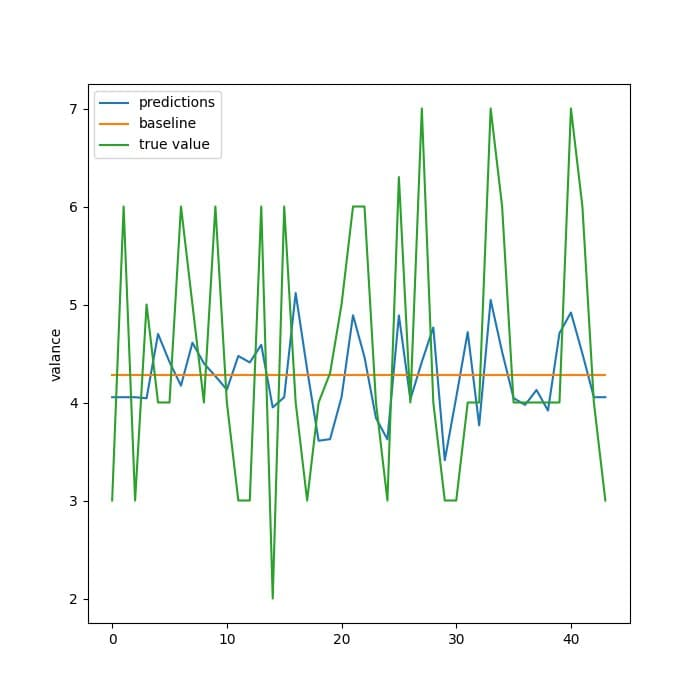
\includegraphics[width=14cm]{figures/results/reg_fit}   
        \caption{Here we can see one of the participants models, using the SVR model, duration of 10 and trained with both keyboard and mouse.}
        \label{fig:reg_fit} 
    \end{figure}

    For our regression models, the results are more inconsistent. On the one hand, we can see that the mean absolute error is usually 
    smaller than 1 for the best models, which is very good when our scale is 0-8. But when we look at the baseline model, 
    we also consistently see that the baseline model has an MAE of around 1. Here \ref{fig:reg_fit} we can see an example of 
    how our model is trying to fit the valance line. The model seems not to predict the extreme valance changes and almost always 
    stays around the 3-5 area, though it can predict some of the peaks and usually is correct in the direction of change of the valance.

    \newpage

    \subsection{Facial Models}

    Our deep learning models managed to achieve much better results compared to the classical models. 
    This improvement makes sense when we consider the data they use. Facial data carries features that are more 
    indicative of a user's emotional state compared to mouse and keyboard features, such as average press duration or mouse angle.

    \begin{figure}[!htp]
        \centering
        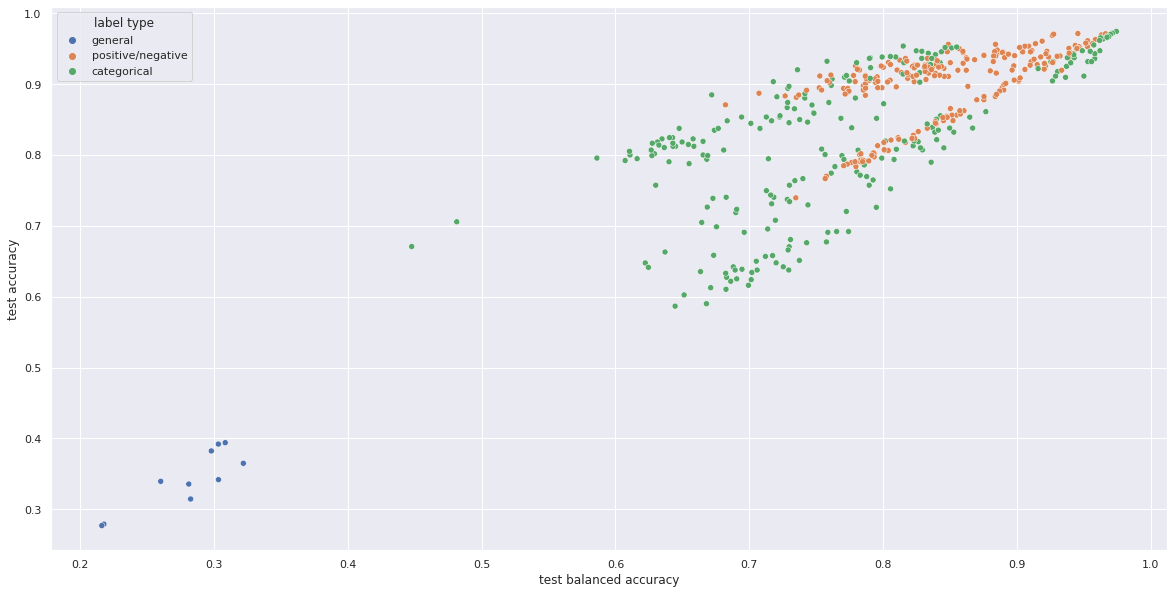
\includegraphics[width=14cm]{figures/results/nn_acc}   
        \caption{We can see the balanced and unbalanced accuracies of all the "Emotion Net Nano" based models we trained in this plot.
        We can also see the colors separating the models into three categories, models predicting positive/negative labels, models predicting
        categorical labels, and the general models that were trained on all the participants at once.}
        \label{fig:nn_acc} 
    \end{figure}

    When we look at the categorical and positive/negative Label types \ref{fig:nn_acc}, we can clearly see an improvement over 
    the classical models, where even the worst of the personal models achieve better performance than the best classical models.
    On the other hand, we can also see that the general models, those trained on all the participants' data, achieve inferior results, 
    even compared to the classical models. On the other hand, we can also see that the general models, 
    those trained on all the participants' data, achieve inferior results, even compared to the classical models when trying 
    to generalize over different people. The inability to generalize facial features is likely due to the minimal data 
    set and our model being very small and simple in terms of trainable parameters. This is not necessarily a bad thing. 
    We intended to create tiny and efficient models that would train on a user's computer and make predictions very easily and quickly.

    \begin{figure}[!htp]
        \centering
        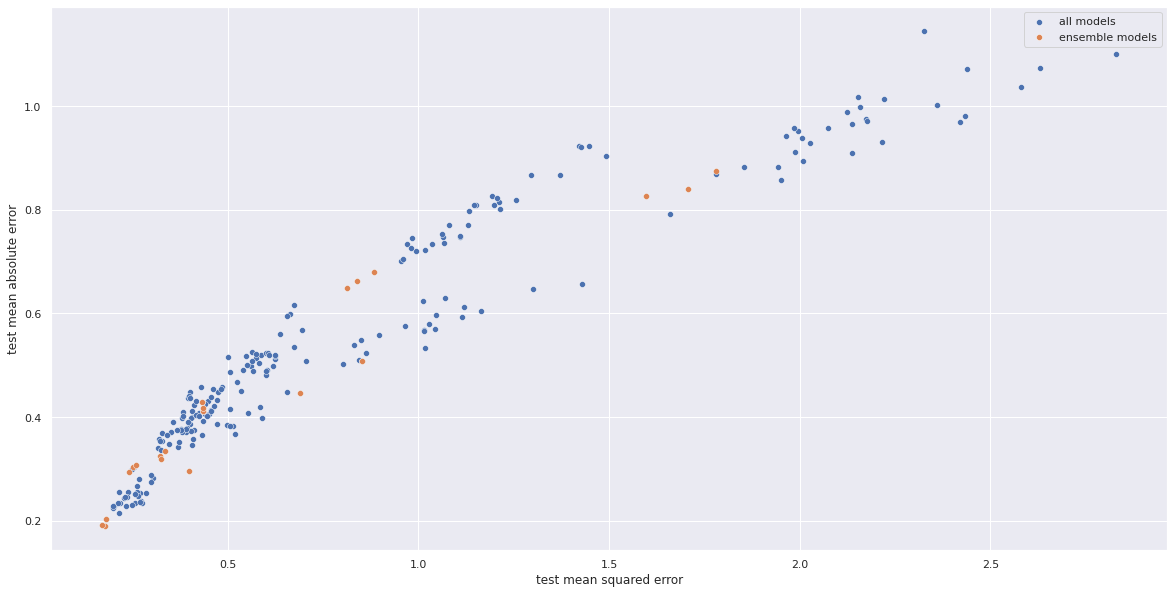
\includegraphics[width=14cm]{figures/results/nn_err}   
        \caption{Here we can see the mean absolute and squared errors of allt he regression models, where the ensemble models are highlated in orange}
        \label{fig:nn_err} 
    \end{figure}


    The story is a bit different when looking at the VAD models \ref{fig:nn_err}. First, we can notice that the variance is very high. 
    Secondly, we have excellent models that achieve a Mean absolute error of less than 0.2, which is much better than the classical models. However, 
    we also have quite a few models that achieve results not much better, even as bad as an MAE of one. Though if we only look at the ensemble models, 
    we can see that they are a little more consistent. We constructed confidence intervals for all the models and just the ensemble models, 
    and with a confidence of 0.95, we can say that all the models are in the range $(0.08, 1)$ and $(0.03, 0.86)$ for ensemble models. Both intervals 
    have incredibly impressive lower bounds, but the upper bound is a little high. 

    \begin{figure}[!htp]
        \centering
        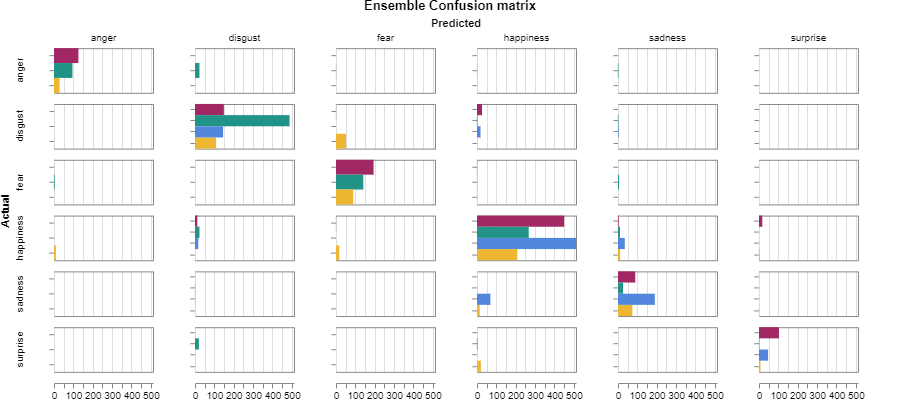
\includegraphics[width=14cm]{figures/results/nn_ensemble_cm}   
        \caption{Confusion matrix describing the predictions of four of the participants.}
        \label{fig:nn_ensemble_cm} 
    \end{figure}

    When looking at the confusion matrix \ref{fig:nn_ensemble_cm}, we can see that the models look relatively consistent, 
    there is some difference between the participants when it comes to the distribution of the labels, 
    as expected, but it seems that each participant's models compensate for this imbalance. Without looking at the 
    problem we are solving, one could easily consider such an effect overfitting, but this is not necessarily the case. 
    Human emotions are very biased in terms of which emotions each of us experiences more, the intensity with which we experience them. 
    This is another reason for why we chose to use personal models so that they might be able to learn these personal biases we have and fit the user better.

    \newpage
    
    \subsection{Ensemble}

    The results of the ensemble were not as we predicted. We thought that combining the best models from each channel can increase the accuracy. 
    We found out that our two approaches of ensemble models mentioned previously in the methodology section \ref{section:methodology_ensemble} 
    did not improve the results. 

    \begin{figure}[!htp]
        \centering
        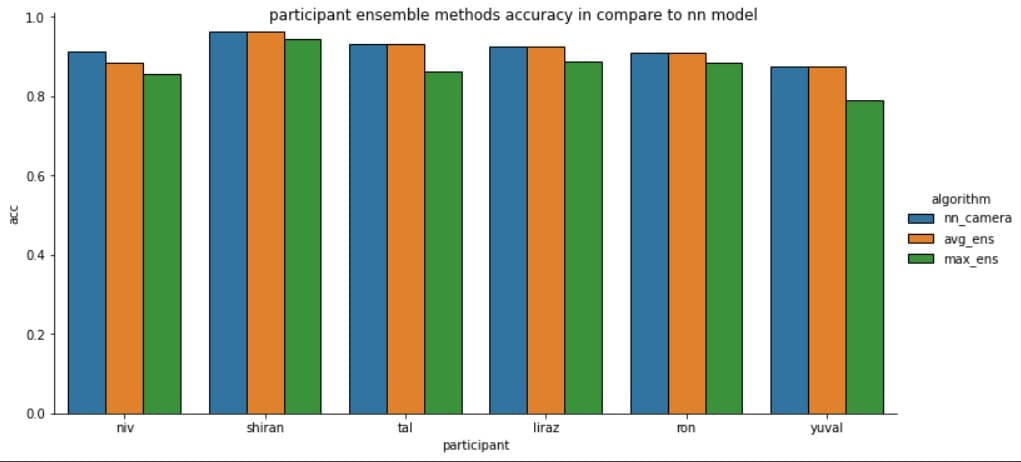
\includegraphics[width=14cm]{figures/results/categorical_ensemble}   
        \caption{Here we can see the ensemble results for the categorical label type.}
        \label{fig:categorical_ensemble} 
    \end{figure}

    As we can see in \ref{fig:categorical_ensemble}, the best accuracy for every participant came from the Neural Network model based on the camera channel. 
    The weighted average approach did not improve the accuracy, but neither reduced (except for 1 participant). 
    We tried to lower the weights a bit for the Neural Network model but received lower accuracy.
    According to the max probability ensemble model we achieved lower accuracy for each participant. 
    We can infer that mouse and keyboard models are sometimes confident about their label even when the label is not correct.

\end{document}